\documentclass{amsart} 
\usepackage{amsmath}
\usepackage{verse}
\DeclareMathOperator*{\argmax}{arg\,max}
\DeclareMathOperator*{\argmin}{arg\,min}
\usepackage{graphicx}
\graphicspath{{./}}
\usepackage[fontsize=14pt]{scrextend}
\usepackage{hyperref}
\usepackage{csvsimple}
\usepackage{epigraph}
\title{Zulf's Hypothesis for Infinite Dimensional Measurement of Human Race April 18 2021}
\author{Zulfikar Moinuddin Ahmed}
\date{\today}
\begin{document}
\maketitle

\section{Reductionist Measurement of Man}

For centuries humanities scholars have chastised scientists for reductionist approaches to the full human being.  Human beings are intrinsically multifaceted and complex, and cannot be reduced to simple models.  I am {\em very sympathetic} to these humanistic scholars. Nothing has incensed me in the past more than reduction of untelligence to a single number and denigrating people by that number, IQ.  I was displeased by the confidence exhibited by {\em The Bell Curve} and spent a great deal of time disseminating Stephen Jay Gould's {\em The Mismeasure of Man}.  

Time has come for me to show a different approach to these problems that have plagued our people the Human Race.

\section{Very High Dimensional Measurements of the Human Being}

Suppose that, rather than taking $p<50$ measurements, ignoring all practical constraints, we were able to take $p=500,000$ measurements.  My colleagues in humanities will admit that if we were able to take $p=500,000$ measurements of a man, let us denote the measurements as $v \in \mathbf{R}^p$ and we had the means to take them for all members $h \in \mathcal{H}$ of the human race every hour for 10 years.  I think such a hypothetical situation would please my humanist colleagues as sufficiently non-reductionist view of both individual human beings and the entire human race.  I leave it to your imagination what each measurement variable ought to be.  They could include such esoteric questions as:  "how many times in your life have you gone to the beach with your friends without ability to swim in Europe and were trying hard to float but had trouble and instead of trying to help you they immediately introduced themselves to beautiful bikini-clad ladies with laughter at your distress?"  I won't go into this one.  Anyway, all sorts of questions that can elucidate your internal and external state is in $v \in \mathbf{R}^p$.

The idea is that we will let $p \uparrow \infty$.  We let our state space $S_p = \mathbf{R}^p$ then approach a separable infinite dimensional Hilbert space $S$.

\section{Generalised Hyperbolic Distribution Hypothesis}

For every $p=1,2,3,\dots$ let $S_p$ be the state space for the set of measurements we will take for the entire Human Race.  We let the measurement be a function $F_p: S_p \rightarrow \mathbf{R}^p$.  We consider each $F_p$ to have a distribution that is a Generalised Hyperbolic Distribution on $\mathbf{R}^p$.  We want to understand the limiting distribution on $S=S_{\infty}$.  We assume this is a GHD as well.  

\section{Zulf's Hypothesis}

The infinite dimensional correlation is a self-adjoint linear operator on the Hilbert space $S$ whose eigenvalues are distributed as the following exact distribution:

\begin{verbatim}
> summary(fit.we)
Asymmetric Generalized Hyperbolic Distribution:

Parameters:
    lambda  alpha.bar         mu      sigma      gamma 
-0.5017696  0.1123917  0.4608804  1.2298894  0.5391586 

Call:
fit.ghypuv(data = ev$values)

Optimization information:
log-Likelihood:                -563.6492 
AIC:                           1137.298 
Fitted parameters:             lambda, alpha.bar, mu, sigma, gamma;  (Number: 5)
Number of iterations:          478 
\end{verbatim} 

And the pictures tell you what it will look like.

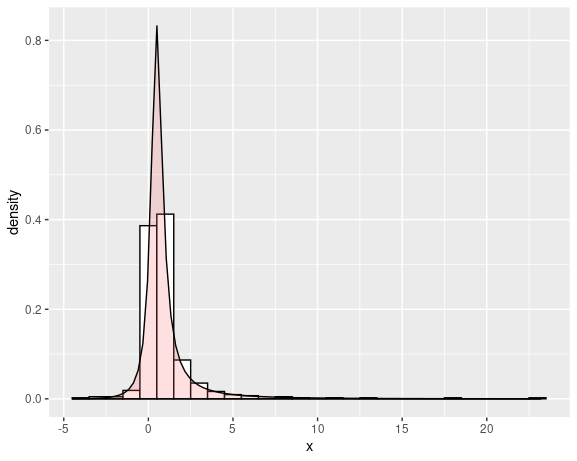
\includegraphics[scale=1.0]{wveig.png}

\section{Need For Operator Theory of Bounded Self-adjoint Operators on a Hilbert Space}

More than a century ago Erik Ivar Fredholm shook the world of mathematics in 1900 with his beautiful proposal of integral operators and infinite dimensional determinants.  It so affected the great David Hilbert that he put aside all his other considerations and worked on the theory of operators on Hilbert Spaces for years.  Just looking at a beautiful continous distribution for the eigenvalues of a Human Values I am simply just amazed by the power of the ideas generated in 1900 by Erik Ivar Fredholm, for this is clearly the limiting distribution of eigenvalues of the correlation matrix of very general infinite dimensional measurements of human race.  I am being quite a bit less precise in this note but sufficiently precise so we understand the natural generalisation to the infinite dimensional situation where mathematicians have worked out a very beautiful theory for self-adjoint operators on a Hilbert space originally for quantum theory.  My Four-Sphere Theory implies that for macroscopic physics we do not need the generality of abstract quantum theory, but here it the generality is supremely clear and applicable.  

\section{Not a Purely Technical Proposal}
Sometimes mathematical people like to generalise situations for the sake of mathematical understanding of hypothetical situations.  Here we claim that this is much more important for Social Science, for there is a natural infinite dimensional structure to Human Race measurements that was hitherto unclear.  One one hand, humanities scholars have been wrong to criticise attempts to produce theories for human race that are simple for pragmatic bounds of social science; on the other hand, their criticism is actually necessary to have an accurate science for Human Race Values and other measuements and here the role of Generalised Hyperbolic (Asymmetric) distributions are quite remarkable.

\end{document}